\begin{pastexam}[label={px:ust-115-ee-ds-33}]{臺聯大電機類 115 學年度 第 33 題}
（單選；2 分）

In graph theory an undirected graph has two kinds of incidence matrices: unoriented and oriented.
The unoriented incidence matrix of an undirected graph is a $n\times m$ matrix B, where $n$ and $m$
are the number of vertices and edges respectively, such that
\[ B_{ij}=\begin{cases}1 & \text{if vertex } v_i \text{ is incident with edge } e_j\\ 0 &
\text{otherwise}\end{cases} \]
An undirected graph (with no self-loops) consisting of 4 nodes and 4 edges is given as followed:

\begin{center}
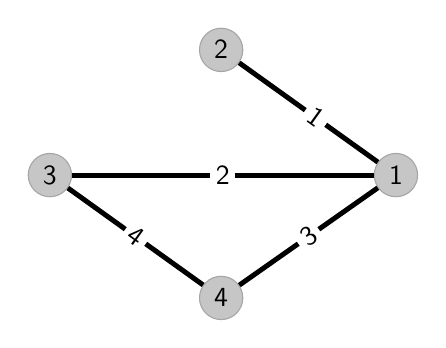
\begin{tikzpicture}[x=1.5cm,y=-1.5cm,
  v/.style={circle,draw=gray!70,fill=gray!45,inner sep=1pt,minimum size=5.5mm,font=\sffamily},
  e/.style={line width=1.8pt},
  w/.style={fill=white,inner sep=2pt,font=\sffamily}]
\node[v] (n2) at (4.55,4.80) {2};
\node[v] (n1) at (6.03,5.86) {1};
\node[v] (n3) at (3.10,5.86) {3};
\node[v] (n4) at (4.55,6.90) {4};
\draw[e] (n2) -- node[w,sloped,pos=0.55] {1} (n1);
\draw[e] (n3) -- node[w] {2} (n1);
\draw[e] (n4) -- node[w,sloped] {3} (n1);
\draw[e] (n3) -- node[w,sloped] {4} (n4);
\end{tikzpicture}
\end{center}

The incidence matrix of the undirected graph above is (e$_1$: (1,2), e$_2$: (1,3), etc.):

\begin{center}
\begin{tabular}{|c|c|c|c|c|}\hline
  & e$_1$ & e$_2$ & e$_3$ & e$_4$\\\hline
1 & 1 & 1 & 1 & 0\\\hline
2 & 1 & 0 & 0 & 0\\\hline
3 & 0 & 1 & 0 & 1\\\hline
4 & 0 & 0 & 1 & 1\\\hline
\end{tabular}
\end{center}

The incidence matrix of a directed graph is a $n\times m$ matrix $B=(b_{ij})$ such that
\[ b_{ij}=\begin{cases}-1 & \text{if edge } e_j \text{ leaves vertex } v_i\\ \phantom{-}1 &
\text{if edge } e_j \text{ enters vertex } v_i\\ \phantom{-}0 & \text{otherwise}\end{cases} \]
The oriented incidence matrix of an undirected graph is the incidence matrix of \textbf{ANY}
orientation of the graph. Check the following oriented incidence matrices of the given graph with
ANY chosen edge direction. Which of the following \textbf{matrix B with the multiplication}:
\textbf{BB$^{\mathrm{T}}$} (T: transpose) will generate a result that is \textbf{different} from the
others?

\medskip
(A)~$\begin{matrix}1&1&1&0\\-1&0&0&0\\0&-1&0&1\\0&0&-1&-1\end{matrix}$\qquad
(B)~$\begin{matrix}-1&1&1&0\\1&0&0&0\\0&-1&0&1\\0&0&-1&-1\end{matrix}$\qquad
(C)~$\begin{matrix}1&-1&1&0\\-1&0&0&0\\0&1&0&-1\\0&0&-1&1\end{matrix}$

\medskip
(D)~$\begin{matrix}-1&-1&-1&0\\1&0&0&0\\0&1&0&-1\\0&0&1&1\end{matrix}$\qquad
(E)~All of the above generate the same results
\end{pastexam}

\begin{pastsoln}
答案是 (E)。

先確認四個矩陣都是這張圖的合法定向關聯矩陣：每一行（一條邊）恰有一個 $+1$、一個 $-1$，而且
出現在那條邊的兩個端點上。 $e_1 = \{1, 2\}$ 在第 1、2 列，$e_2 = \{1, 3\}$ 在第 1、3 列，
$e_3 = \{1, 4\}$ 在第 1、4 列，$e_4 = \{3, 4\}$ 在第 3、4 列，(A)--(D) 都符合，只是邊的方向不同。

再看 $BB^{\mathrm T}$ 的第 $(i, j)$ 項：
\[
(BB^{\mathrm T})_{ij} = \sum_{k=1}^{m} b_{ik}\, b_{jk} .
\]
\begin{itemize}
\item $i = j$：$b_{ik}^2 = 1$ 恰好在 $v_i$ 是 $e_k$ 的端點時成立，所以 $(BB^{\mathrm T})_{ii} =
\deg(v_i)$。
\item $i \ne j$：$b_{ik} b_{jk} \ne 0$ 要 $v_i$、$v_j$ 都是 $e_k$ 的端點，也就是 $e_k$ 連接
$v_i, v_j$；這時兩個值一正一負，乘積是 $-1$，和方向無關。 沒有重邊，所以
$(BB^{\mathrm T})_{ij} = -1$（相鄰）或 $0$（不相鄰）。
\end{itemize}
因此 $BB^{\mathrm T} = D - A$（度數矩陣減鄰接矩陣，叫圖的 Laplacian），完全不看方向。 這張圖的
度數是 $\deg(1) = 3$、$\deg(2) = 1$、$\deg(3) = 2$、$\deg(4) = 2$，四個選項算出來都是
\[
BB^{\mathrm T} = \begin{pmatrix} 3 & -1 & -1 & -1 \\ -1 & 1 & 0 & 0 \\ -1 & 0 & 2 & -1 \\ -1 & 0 & -1 & 2 \end{pmatrix} .
\]
以 (A) 驗算第 $(1,3)$ 項：第 1 列 $(1, 1, 1, 0)$ 和第 3 列 $(0, -1, 0, 1)$ 的內積是 $-1$；第
$(3,3)$ 項：$0 + 1 + 0 + 1 = 2$。 其他項同理。

所以 (A)--(D) 都相同，答案是 (E)。
\end{pastsoln}
